\begin{frame}
  \frametitle{Probleem: Gelukkige Getallen (VPW2011)}
  \begin{center} \large\bfseries
    De \emph{opvolger} van een getal is de som van zijn cijfers.
  \end{center}
  \vskip4mm
  \[
    \begin{array}{r@{}c@{}lcccccc}
      \mathrm{opvolger}(&11&) & = & 1^2 + 1^2 & = & 1 + 1 & = & 2 \\
      \mathrm{opvolger}(&49&) & = & 4^2 + 9^2 & = & 16 + 81 & = & 97 \\
      \mathrm{opvolger}(&123&) & = & 1^2 + 2^2 + 3^2 & = & 1 + 4 + 9 & = & 14
    \end{array}
  \]
\end{frame}

\begin{frame}
  \frametitle{Probleem: Gelukkige Getallen (VPW2011)}
  \begin{center}
    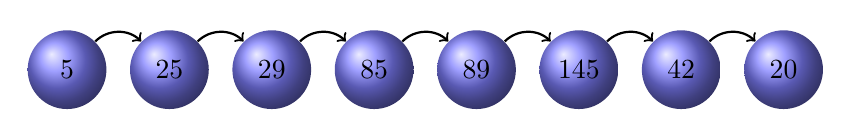
\begin{tikzpicture}[node/.style={ball color=blue!50,circle,minimum size=1cm}]
      \foreach[count=\i] \c in {5,25,29,85,89,145,42,20} {
        \pgfmathparse{\i*1.3}\let\cx\pgfmathresult
        \node[node] (node \i) at (\cx,0) {\c};
      }
      \foreach \i in {1,...,7} {
        \pgfmathparse{int(\i+1)}\let\j\pgfmathresult
        \draw[->,thick] (node \i.north east) to [bend left=45] (node \j.north west);
      }
    \end{tikzpicture}
  \end{center}
  \vskip5mm
  \begin{center}
    \large Ketting van opvolgers
  \end{center}    
\end{frame}

\begin{frame}
  \frametitle{Probleem: Gelukkige Getallen (VPW2011)}
  \begin{center} \Large\bfseries
    \emph{Gelukkig getal}: ketting eindigt op 1.
  \end{center}

  \begin{columns}
    \column{.5\linewidth}
    \begin{center}
      \begin{tikzpicture}[transform shape,scale=0.5,
                          node/.style={ball color=blue!50,circle,minimum size=1cm},
                          arrow/.style={-{Straight Barb[length=1pt]}}]
        \path[use as bounding box] (-1,-3) rectangle (10,3);
        \foreach[count=\i] \c in {7,49,97,130,10,1} { 
          \pgfmathparse{\i*1.25}\let\x\pgfmathresult
          \node[node] (node \i) at (\x,0) {\c};
        }

        \foreach \i in {1,...,5} {
          \pgfmathparse{int(\i+1)}\let\j\pgfmathresult
          \draw[arrow] (node \i) to [bend left=30] (node \j);
        }
        \draw[arrow] (node 6) to [loop right] (node 6);
      \end{tikzpicture}
    \end{center}
    \begin{center} 7 is gelukkig \end{center}

    \column{.5\linewidth}
    \begin{center}
      \begin{tikzpicture}[transform shape,scale=0.5,
                          node/.style={ball color=blue!50,circle,minimum size=1cm},
                          arrow/.style={-{Straight Barb[length=1pt]}}]
        \path[use as bounding box] (0,-3) rectangle (11,3);

        \foreach[count=\i] \c in {5,25,29,85} { 
          \pgfmathparse{\i*1.25}\let\x\pgfmathresult
          \node[node] (node \i) at (\x,0) {\c};
        }
        \foreach[count=\i] \c in {89,145,42,20,4,16,37,58} {
          \pgfmathparse{int(\i+4)}\let\j\pgfmathresult
          \pgfmathparse{180-360/8*(\i-1)}\let\angle\pgfmathresult
          \node[node,xshift=8.25cm] (node \j) at (\angle:2cm) {\c};
        }
        \foreach \i in {1,...,11} {
          \pgfmathparse{int(\i+1)}\let\j\pgfmathresult
          \draw[arrow] (node \i) to [bend left=30] (node \j);
        }
        \draw[arrow] (node 12) to [bend left=30] (node 5);
      \end{tikzpicture}
    \end{center}
    \begin{center} 5 is ongelukkig \end{center}
  \end{columns}
\end{frame}

\begin{frame}
  \frametitle{Probleem: Gelukkige Getallen (VPW2011)}
  \begin{center} \Large
    Opgave: schrijf een functie {\tt gelukkig(n)} die nagaat
    of {\tt n} gelukkig is.
  \end{center}
\end{frame}

\begin{frame}
  \frametitle{Eerste poging}
  \code[width=.6\linewidth]{first-attempt.js}
  \visible<2>{
    \begin{center}
      Kan geen ongelukkige getallen detecteren: oneindige lus.
    \end{center}
  }
\end{frame}

{
\newcommand{\drawgraph}[1]{{
  \let\activenode#1
  \foreach[count=\i] \c in {5,25,29,85} { 
    \pgfmathparse{\i*1.25}\let\x\pgfmathresult
    \pgfmathparse{ifthenelse(equal(\i,\activenode),"selected node","node")}\let\s\pgfmathresult
    \node[\s] (node \i) at (\x,0) {\c};
  }
  \foreach[count=\i] \c in {89,145,42,20,4,16,37,58} {
    \pgfmathparse{int(\i+4)}\let\j\pgfmathresult
    \pgfmathparse{180-360/8*(\i-1)}\let\angle\pgfmathresult
    \pgfmathparse{ifthenelse(equal(\j,\activenode),"selected node","node")}\let\s\pgfmathresult
    \node[\s,xshift=8.25cm] (node \j) at (\angle:2cm) {\c};
  }
  \foreach \i in {1,...,11} {
    \pgfmathparse{int(\i+1)}\let\j\pgfmathresult
    \draw[arrow] (node \i) to [bend left=30] (node \j);
  }
  \draw[arrow] (node 12) to [bend left=30] (node 5);
}}

\begin{frame}
  \begin{center}
    \begin{tikzpicture}[node/.style={ball color=blue!50,circle,minimum size=1cm},
                        selected node/.style={node,ball color=green!50},
                        arrow/.style={-latex}]
      \foreach[count=\slideindex] \i in {1,...,12,5,6,...,12} {
        \only<\slideindex>{
          \drawgraph{\i}
        }
      }
    \end{tikzpicture}
  \end{center}
\end{frame}
}

\begin{frame}
  \begin{center} \Large
    Hoe lossen we dit best op?
  \end{center}
\end{frame}

{
\newcommand{\drawgraph}[1]{{
  \let\activenode#1
  \foreach[count=\i] \c in {5,25,29,85} { 
    \pgfmathparse{\i*1.25}\let\x\pgfmathresult
    \pgfmathparse{ifthenelse(\i<\activenode,"visited node",ifthenelse(equal(\i,\activenode),"selected node", "node"))}\let\s\pgfmathresult
    \node[\s] (node \i) at (\x,0) {\c};
  }
  \foreach[count=\i] \c in {89,145,42,20,4,16,37,58} {
    \pgfmathparse{int(\i+4)}\let\j\pgfmathresult
    \pgfmathparse{180-360/8*(\i-1)}\let\angle\pgfmathresult
    \pgfmathparse{ifthenelse(\j<\activenode,"visited node",ifthenelse(equal(\j,\activenode),"selected node", "node"))}\let\s\pgfmathresult
    \node[\s,xshift=8.25cm] (node \j) at (\angle:2cm) {\c};
  }
  \foreach \i in {1,...,11} {
    \pgfmathparse{int(\i+1)}\let\j\pgfmathresult
    \draw[arrow] (node \i) to [bend left=30] (node \j);
  }
  \draw[arrow] (node 12) to [bend left=30] (node 5);
}}

\begin{frame}
  \begin{center}
    \begin{tikzpicture}[node/.style={ball color=blue!50,circle,minimum size=1cm},
                        selected node/.style={node,ball color=green!50},
                        visited node/.style={node,ball color=red!50},
                        arrow/.style={-latex}]
      \foreach[count=\slideindex] \i in {1,...,12} {
        \only<\slideindex>{
          \drawgraph{\i}
        }
      }
    \end{tikzpicture}
  \end{center}
\end{frame}
}

\begin{frame}
  \frametitle{Gebruik makend van verzamelingen}
  \code[width=.9\linewidth]{with-set.js}
\end{frame}


%%% Local Variables: 
%%% mode: latex
%%% TeX-master: "slides"
%%% End: 
